\chapter{Specifications}

\section{Functional Description}

The AHB-Lite PLIC IP core is a fully parameterised Platform-Level Interrupt
Controller, featuring a single AHB-Lite Slave interface and support for a user-defined number of both Interrupt Sources and Targets.

The purpose of the PLIC core is to connect multiple interrupt sources to
one or more interrupt targets. The core supports a programmable number
of simultaneous pending interrupt requests per source and individual routing of those interrupt requests to each target.

Per the \href{https://github.com/riscv/riscv-isa-manual/blob/master/release/riscv-privileged-v1.9.1.pdf}{RISC-V Privileged Architecture Instruction Set specification (v1.9.1)}, the core performs full interrupt prioritisation of each interrupt source; each may be assigned a separate priority and enabled per target via a matrix of interrupt enable bits. Further, an optional priority threshold per target may be defined to mask lower priority interrupts.

To reduce latency, the PLIC core presents all asserted interrupts to the target in priority order, queuing them so that a software interrupt handler can service all pending interrupts without the need to restore the interrupted context.

For illustration, a simplified example system using the PLIC core is shown below:

\begin{figure}[!htb]
	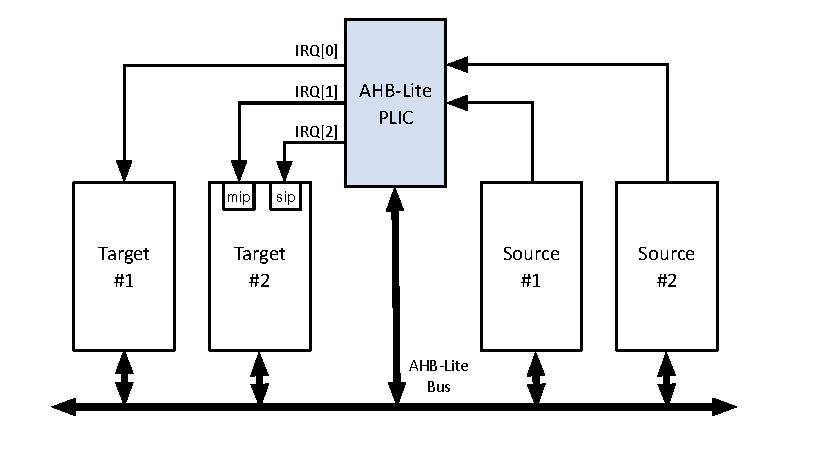
\includegraphics{assets/img/plic-system}
	\caption{PLIC System Diagram}
	\label{fig:SYSDIAG}
\end{figure}

\section{Interrupt Handling Handshake}

The Roa Logic implementation of the handshake between Interrupt source,
target and PLIC is illustrated below, and described in further detail in
the subsequent sections:

\begin{figure}[!htb]

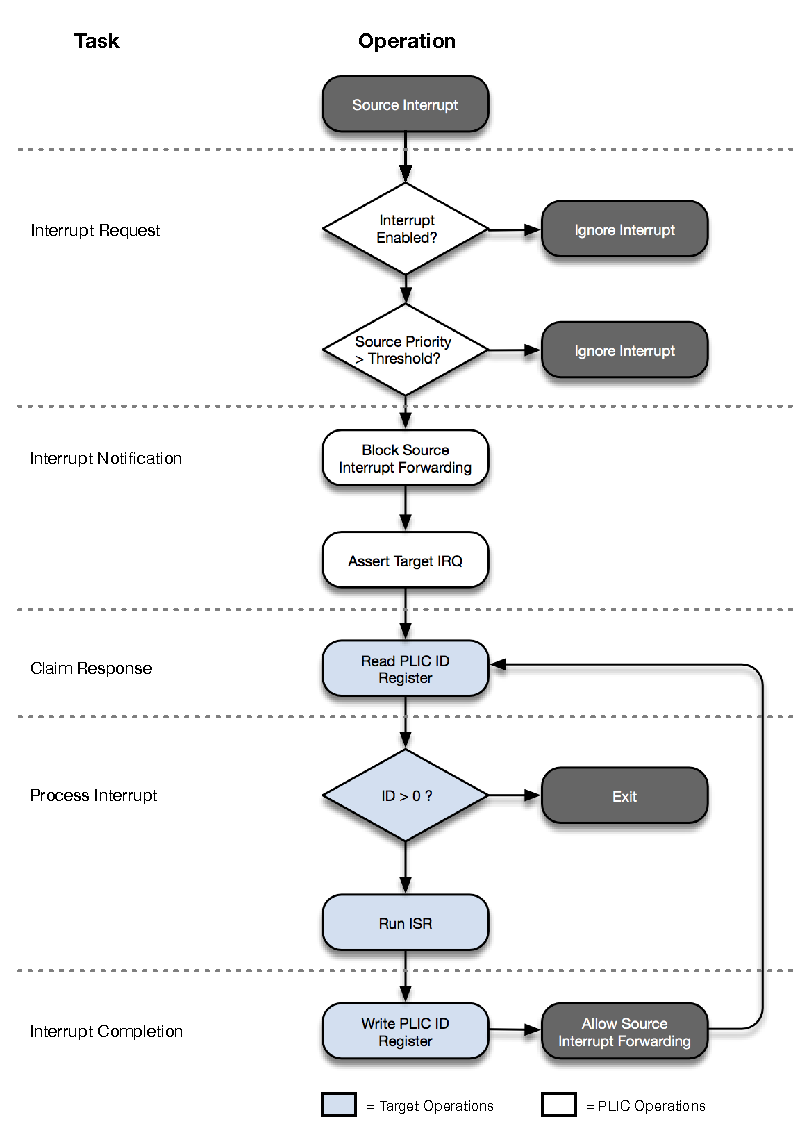
\includegraphics{assets/img/plic-handshake}
\caption{Interrupt Handling handshake}
\label{fig:HANDSHAKE}
\end{figure}

\subsection{PLIC Configuration}

A matrix of Interrupt Enable vectors -- one IE register per target --
determines which target processes the interrupts from which source.

Each Interrupt Source attached to the PLIC is then assigned a Priority
Level - an unsigned integer that determines the relative priority of
the interrupt source. The greater the integer, the greater the priority
level. A Priority Threshold per target may also be defined to mask lower
priority interrupts such that interrupts will only be presented to a
target if the assigned Priority Level is greater than the Priority Threshold.

In addition each source is automatically assigned an Interrupt Identifier
(\texttt{ID}) -- an unique unsigned integer. This identifier determines
interrupt priority when 2 or more interrupts with the same priority
level are asserted. The lower the \texttt{ID} assigned to the source,
the greater the interrupt priority.

\subsection{Interrupt Request}

A source asserts an interrupt request to the PLIC. The PLIC validates
the request by first checking if an interrupt enable bit is set for each
target and if the priority of the interrupt source exceeds any defined
Interrupt Priority Threshold. If these conditions do not hold, the
Interrupt Request is deemed invalid and stalled pending updates to the interrupt enable and/or priority threshold bits. 

The PLIC also determines if a previous interrupt request has been made
by the same source. If an interrupt is defined as level triggered and
has already been asserted but not yet serviced, the request is ignored.
If an interrupt is defined as edge triggered and has already been
asserted but not yet serviced, the request is queued by incrementing a
Interrupt Pending counter by one. The depth of this counter is
parameterised.

If the request is deemed valid the request is forwarded to the
appropriate target. In the case of queued edge-triggered requests, the
interrupt pending counter is decremented by one immediately upon claim of the interrupt by the target.

\subsection{Interrupt Notification}

A target is notified of an interrupt request by the assertion of the IRQ
output for the relevant target. The PLIC also blocks the forwarding of
any further requests from the interrupt source until the asserted
request is serviced.

On each clock cycle the ID register is loaded with the unique identifier
of the highest priority interrupt to be processed.

\subsection{Claim Response} \label{sec:claim-response}

A target makes an interrupt claim response by reading the ID register,
which also notifies the target of the interrupt source to service. The
PLIC de-asserts the IRQ output for the target in response to the claim.
unless another, lower priority, interrupt is still pending.

\subsection{Interrupt Handler}

If the ID read is greater than zero, the target services the identified
interrupt source. If the ID read is zero, this indicates no outstanding
pending interrupts remain and the handler may terminate.

\subsection{Interrupt Completion}

Once an interrupt has been serviced, completion is signalled to the PLIC
by writing to the ID register. The act of writing to the register is the
completion notification; the value written is irrelevant.

On receiving the completion notification the PLIC will again allow
interrupts to be forwarded from the corresponding source.

The Interrupt Handler may then exit, however it is possible a new
interrupt request may have been asserted while the handler was running.
To reduce latency the handler may instead determine if a new interrupt
has been received and if so again claim the interrupt (See earlier). In this
way the interrupt handler can service all interrupts without the need to
restore the interrupted context.
